\section{Performance}
We have included the following two versions of our program:
\begin{itemize}
\item The \verb!/Cuda/! directory contains our finished program which fully runs on CUDA.
\item The \verb!/OrigImpl/! directory contains our fully transformed CPU implementation which runs with OpenMP.
\end{itemize}
\subsection{Runtime}
\subparagraph{Setup:} All tests were performed on gpu2 of the GPU servers.


\subparagraph{Results:} 

30 run tests were run on each of the following program versions, with the total runtime (in microseconds) averaged:
\begin{itemize}
\item Original CPU implementation. Runtime average: 2450300.
\item Original CPU implementation with openmp on outer loop. Runtime average: 220008 .
\item Fully modified CPU implementation with openmp on parallel loops. Runtime average: 476647.
\item Final CUDA implementation. Runtime average: 390135.

Figure \ref{fig_res} shows a plot of the runtime in each test in the four configurations.
\end{itemize}
\begin{figure}[H]
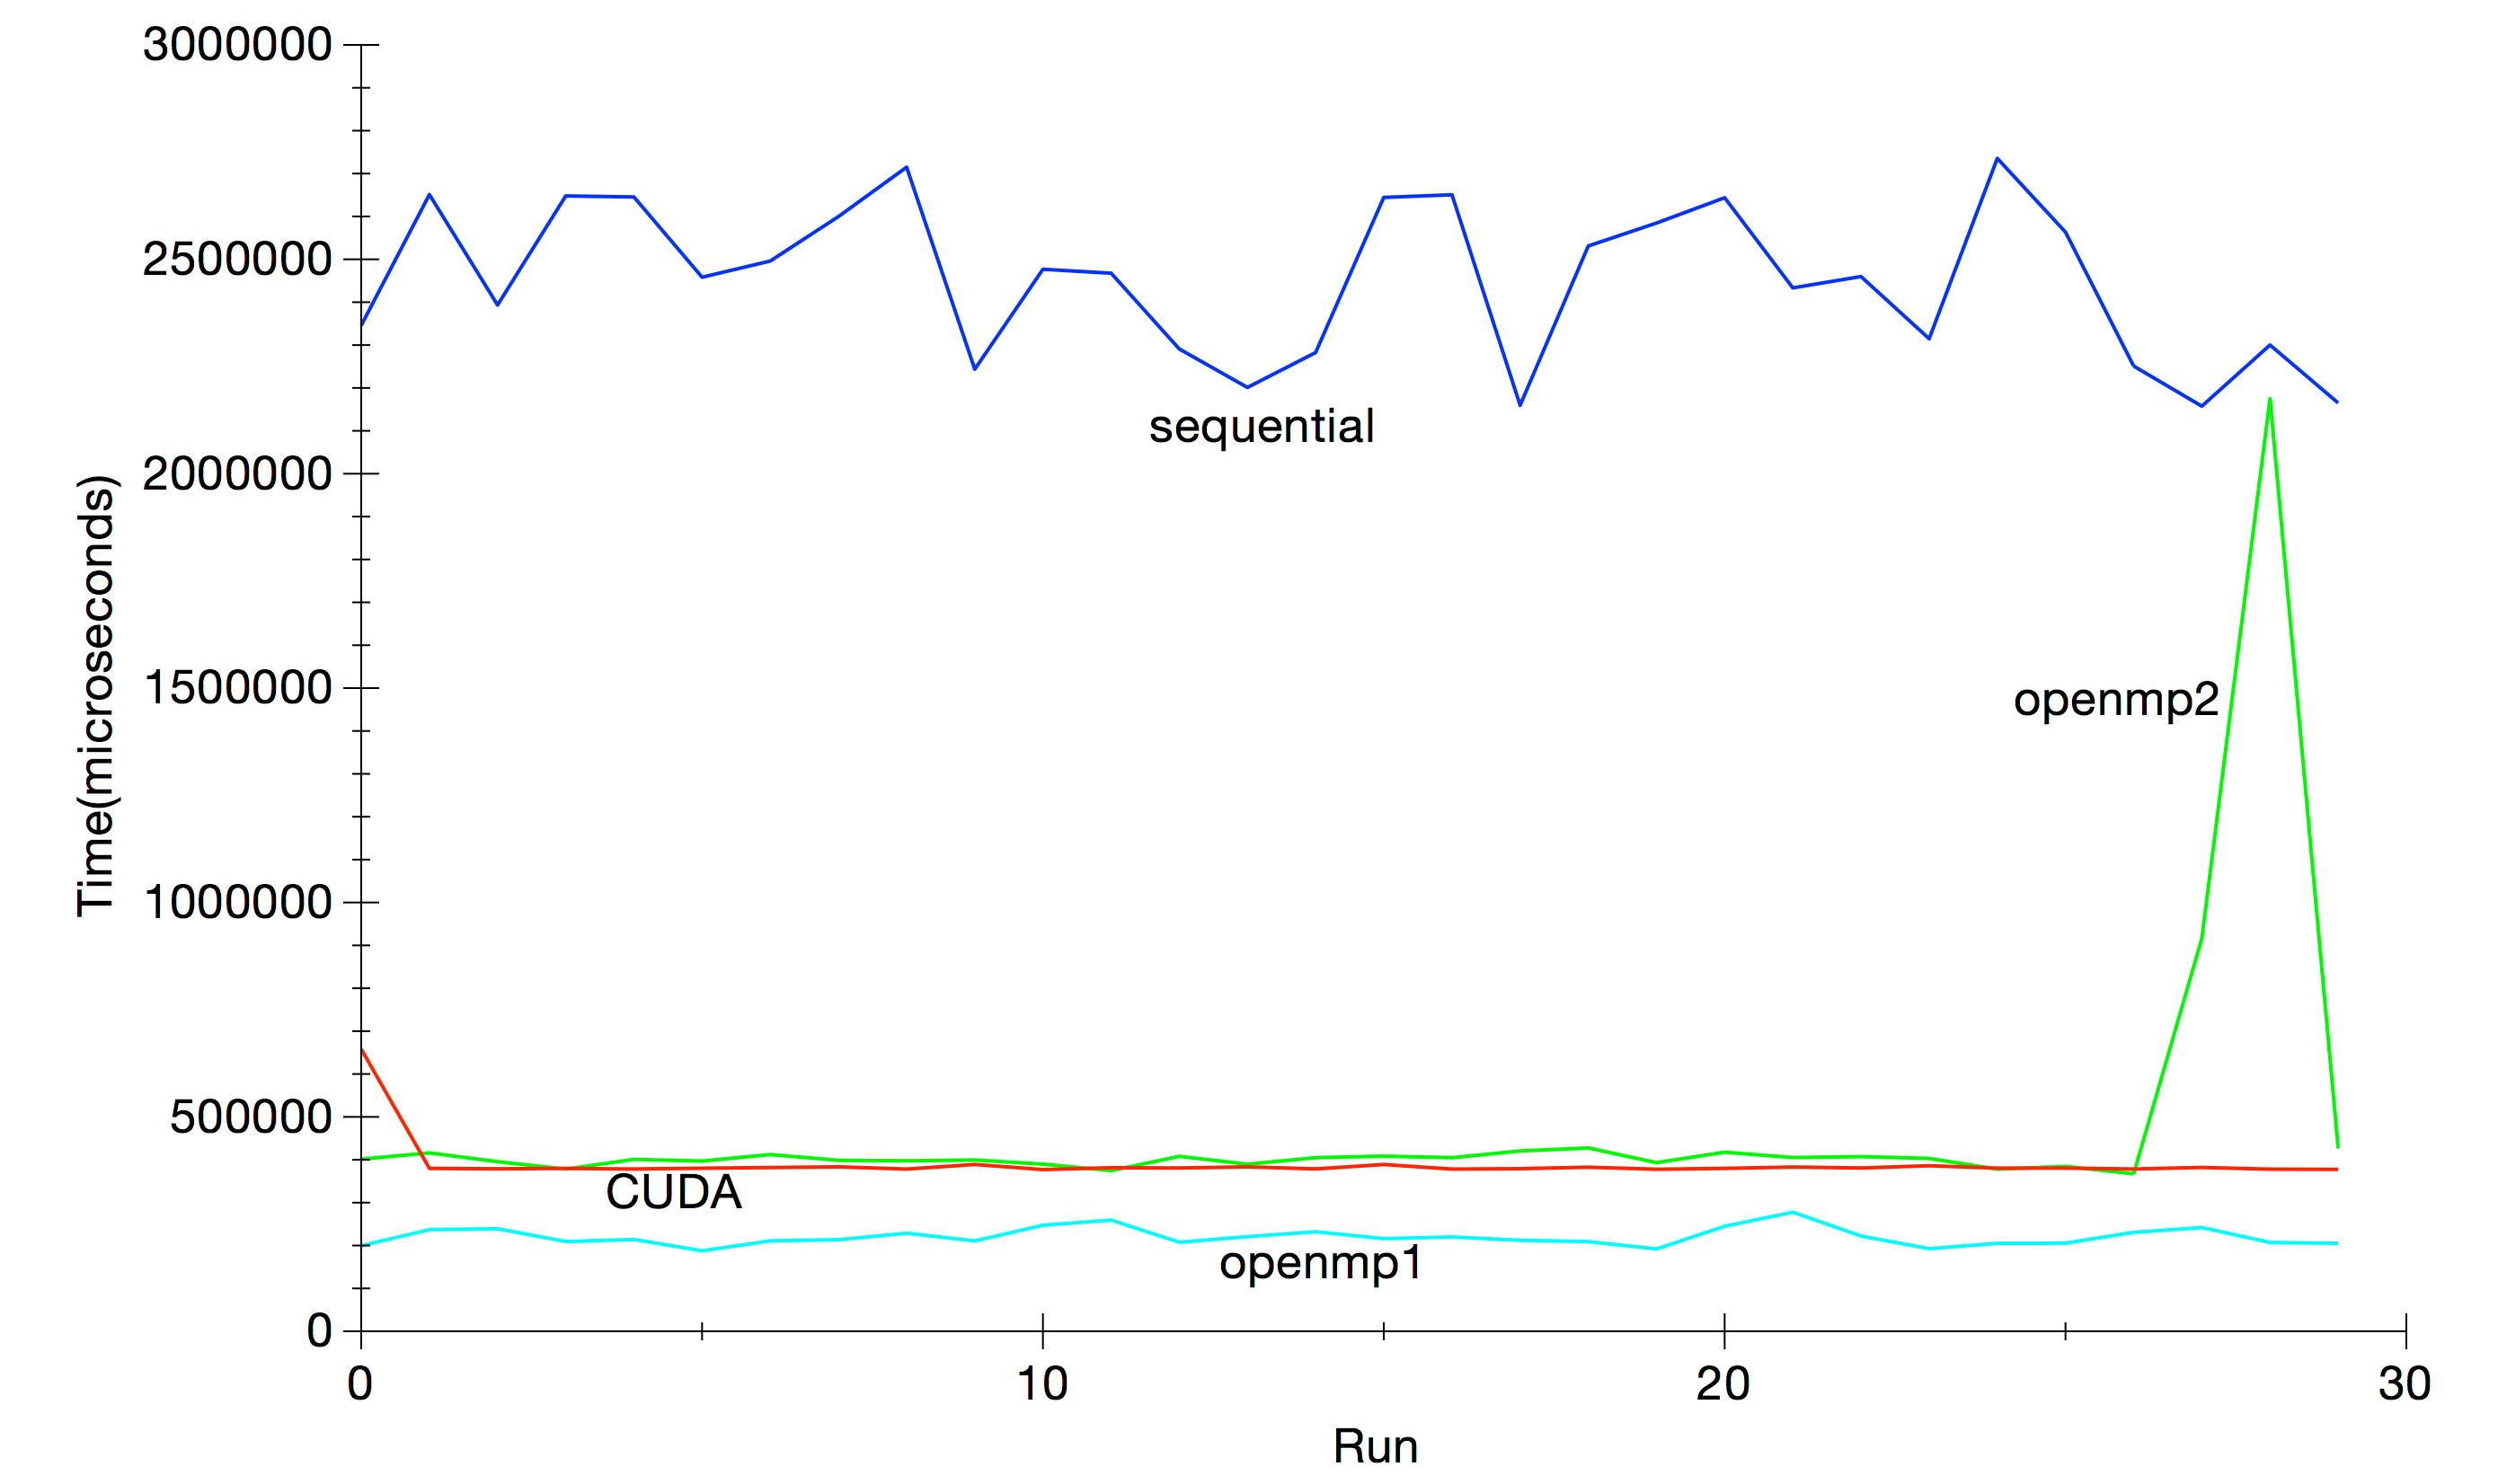
\includegraphics[width=150mm]{results_plot} 
\caption{Runtimes of the four program versions; sequential: original CPU implementation, openmp1: original CPU implementation with openmp on outer loop, openmp2: fully modified CPU implementation with openmp on parallel loops, and CUDA: final CUDA implementation.}
\label{fig_res}
\end{figure}



\subparagraph{Comments:} As expected the original CPU implementation has the highest runtime average by a recognizable margin. The parallelized versions of the code (with CUDA and openmp) have very similar runtimes, but the CUDA implementation has a lower runtime average due to an outlier in the openmp version runtimes. The orriginal CPU implementation with openmp on outer loop has the lowest runtime average, possible reasons are fewer overhead and faster memory access velocity of CPU over GPU. A lower runtime of the CUDA parallel version over the openmp one could be expected in a larger data set.

\subsection{Validation}
The results obtained in all tests were valid.
